\chapter{Software Architecture}
\label{ch:Software_Architecture}

In order to rework the whole project and to increase performance and portability, a new fundamental software architecture was introduced. The main principle of this architecture is to seperate the preprocessing and handling of the data and the distribution to the final application. In contrast to the old solution the data can now be preprocessed more efficiently and send to another component in a generic way. This component is responsible for the distribution of the data to the final application.

\begin{figure}[H]
    \centering
    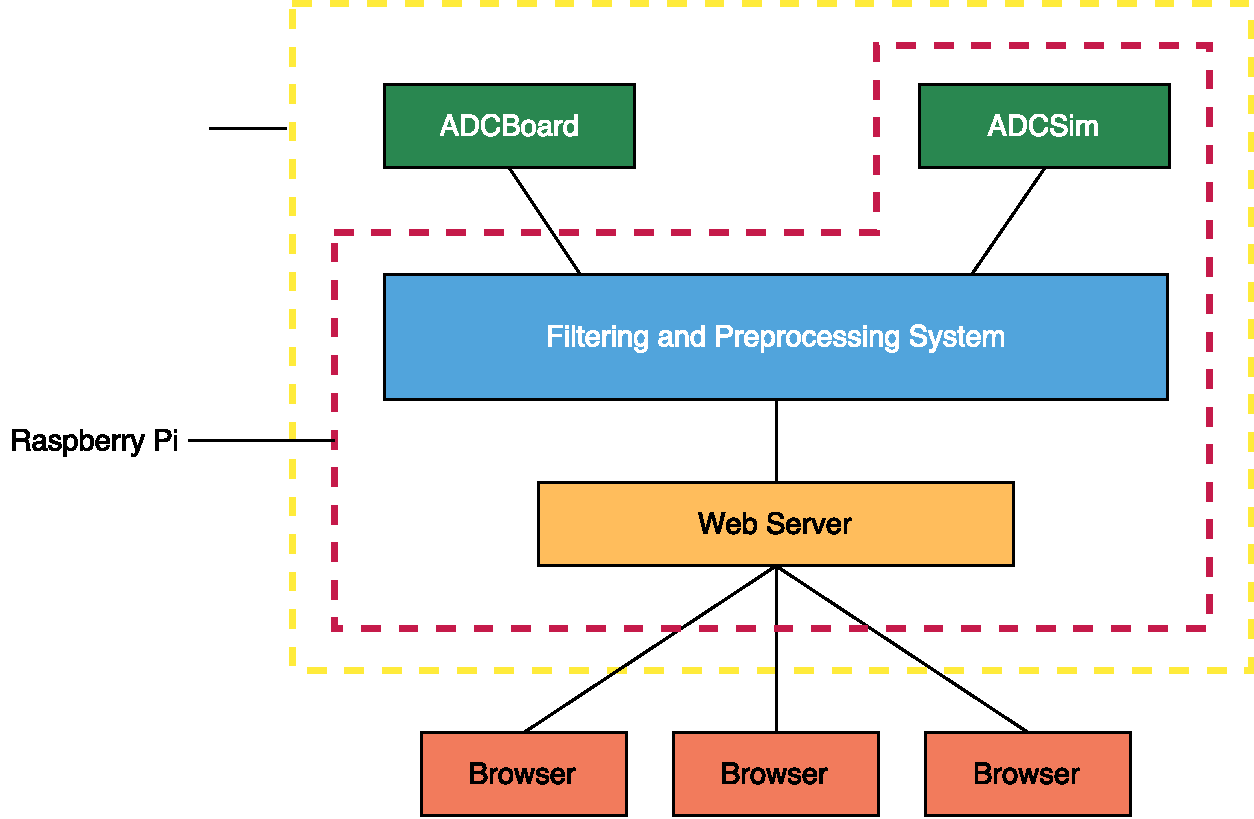
\includegraphics[width=15cm,keepaspectratio]{software_architecture}
    \caption{GRAMOC Software Architecture}
    \label{fig:software_architecture}
\end{figure}

\section{Input}

To process data there must be a source from which the program can obtain its data. In the case of GRAMOC the data are readouts from a gradient magnetometer, theese readouts are split into six channels and transmitted via a custom circuit board. There are two ways how to retrieve the data needed to visualize it, first the custom circuit board called ADCBoard and second a simulator that generates random data.

\subsection{ADC Board}

This is the component that handles analog to digital conversion, hence ADC board. This circuit board receives analog data from the sensor in six channels. The first three channels being the magnetic field and the last three the gradients.

\subsection{Simulator}

To simplify the whole development process a simple way of data generation had to be created. Therefore a small application written in C++ was built. The main feature of the so-called ADCSim, whichs stands for ADC Simulator, is the seamless interchangeability with the real ADC Board. 

\section{Abstraction Layer}

% add subsections for technologies used

\section{Data Distribution}
